\chapter{Problém množinového pokrytia a výber génov}
\label{chap:setcover}
V predchádzajúcej kapitole sme predstavili základné prvky nášho programu ktorý, dostane na vstupe súbor, 
popisujúci evolučnú históriu a na výstupe danú históriu vykreslí.
Problém nastane, pokiaľ sa v histórii nachádza príliš veľa génov. Výsledný vygenerovaný obrázok sa stáva neprehľadným, 
a získanie informácie z neho obtiažne. 
Potrebujeme teda vybrať iba niektoré gény na zobrazenie tak, aby na obrázku zostali zachované podstatné informácie.
V tejto kapitole si predstavíme spôsob, akým môžme automaticky vyberať, ktoré gény zobrazíme.
V našej metóde využijeme \emph{Problému množinového pokrytia} pričom implementujeme dva algoritmy, ktoré riešia daný problém.
\section{Výber génov}
Najpodstatnejšou informáciou pri analýze evolučnej histórie je pre nás to, aké udalosti sa v nej odohrali. 
Budeme sa teda snažiť nájsť podmnožinu všetkých génov tak, aby všetky udalosti ostali na obrázku zachované.
Zvyšné gény následne z obrázku odstránime, čo môže viesť k strate informácie, ktorú považujeme za menej podstatnú, 
ako napríklad, koľko a ktoré gény sa nachádzajú v danej histórii, ako aj koľko a ktoré gény sú ovplyvnené jednotlivými udalosťami.
\subsection{Blok}\label{blok}
Aby sme formálne zadefinovali problém výberu génov, zavedieme pojem bloku. Tento pojem sa vzťahuje na jednu konkrétnu dvojicu krok a jeho predchodca.
\emph{Blok} predstavuje postupnosť génov, ktoré sa pred aj po zmenách, medzi krokom a jeho predchodcom, nachádzali vedľa seba v rovnakom poradí, a jednotlivé gény nemenili
svoju orientáciu. Jedná sa teda o súvislý
úsek DNA, ktorý počas kroku nebol prerušený.
Ak sa pri delécii alebo inzercii odobralo alebo pridalo niekoľko génov, ktoré tvoria súvislý úsek, tvoria jeden blok. 
Gény naľavo a na pravo od týchto zmazaných resp. vložených génov budú tvoriť ďalšie dva bloky.
Pri duplikácii gény tvoria blok, ak sa nachádzali pri sebe pred duplikáciou a rovnako aj po nej vo všetkých zduplikovaných inštanciách.
Pri inverzii tvoria jeden blok gény, ktorým sa zmení orientácia, t.j. Napr blok génov (4,5,-6) bude po inverzii vyzerať ako (6,-5,-4).
Ukážka evolučnej histórie so zobrazenými blokmi je na obrázku \ref{obr:bloky},
v hornej vetve vidíme blok duplikácie, kedy z jedného bloku vznikli dva totožné bloky.
Pre každú vetvu speciácie sa hľadajú bloky medzi predkom a novým druhom zvlášť.

Pre každú dvojicu krok $k$ a jeho predchodca $k_p$, bez ohľadu na to, koľko evolučných udaostí sa medzi nimi odohralo, nájdeme kroky nasledovním spôsobom.
Každý gén $g_i$ z kroku $k_p$ vložíme do nového bloku $b_gi$, každému génu v bloku $k$, ktorý má predka v bloku $k_p$ priradíme rovnaký blok, ako má jeho predok.
Ak má gén $-g_i$ z bloku $k$ predka $g_i$ v bloku $k_p$, a $g_i$ má priradený blok $b_gi$, tak génu $-g_i$ priradíme blok $-b_gi$. 
Génom v $k$ ktoré nemajú predka priradíme nové bloky.
Každú dvojicu blokov $b1$ a za ním nasledujúci $b2$ z $k_p$ spojíme do jedného bloku ak:
Blok $b1$ ani $b2$ a ani blok $-b1$ alebo $-b2$ sa nenachádza v kroku $k$, teda došlo k delécii a bloky môžme spojiť.
Ak sa v kroku $k$ nachádza blok $b1$, vždy za ním nasleduje $b2$, a naopak bloku $b2$ vždy predchádza blok $b1$, tak isto, po bloku $-b2$ musí
vždy nasledovať $-b1$, a bloku $-b1$ vždy predchádza blok $-b2$ , to nám zaručí že bloky (a teda gény v nich) sa počas udalosti vždy nachádzali vedľa seb.

Ked bloky $b1$ a $b2$ spojíme do bloku $b1$ v $k_p$, spoja sa do bloku $b1$ aj v $k$ a bloky $-b2$ a $-b1$ sa spoja do bloku $-b1$ .
Týmto spôsobom prechádzame bloky v kroku $k_p$, pokiaľ dochádza k spojeniam blokov. Na strane $k$ potom pospájame susedné bloky,
ktoré vznikli inzerciou - to sú tie bez predka na strane $k_p$.

\begin{figure}[t]
 \centering
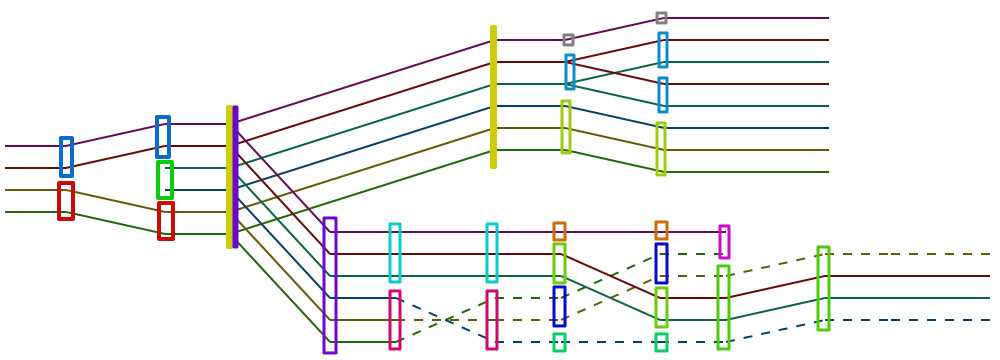
\includegraphics[width=1\textwidth]{images/bloky}
\caption{Ukážka blokov.}\label{obr:bloky}
\end{figure}


\subsubsection{Pokrytie blokov}
Blok považujeme za pokrytý pokiaľ sa na obrázku vyskytuje aspoň jeden gén patriaci do daného bloku.
Pokrytie všetkých blokov jednej dvojice krok a predchodca kroku nám zaručí zobrazenie všetkých udalostí, ktoré sa medzi týmito krokmi vyskytli.
Musíme preto nájsť také gény, ktoré pokryjú všetky bloky v kompletnej evolučnej histórii,
a tým zaistiť zobrazenie všetkých udalostí vo výslednom zobrazení. 
Ako cieľ si zvolíme, aby bola vybraná množina génov čo najmenšia.
\section{Problém množinového pokrytia}
Ako ukážeme nižšie, problém výberu génov úzko súvisí s dobre známym problémom množinového pokrytia.
\paragraph{Definícia}
Máme dané univerzum $U$, ktoré obsahuje $n$ prvkov, a systém jeho podmnožín \(S=\{ P_i : P_i \subseteq U \}\), 
ktorý pokrýva celé univerzum, t.j. \(\cup_{P_i \epsilon S} P_i = U\).
Cieľom je vybrať čo najmenšiu množinu podmnožín \(C \subseteq S\),
 ktorá tiež pokryje celé univerzum \(\cup_{P_i \epsilon C} P_i = U \) .
Problém množinového pokrytia (anglicky Set Cover Problem), ďalej len \emph{PMP}. patrí medzi NP-úplne problémy.\cite{Karp}
\paragraph{Príklad}
Pre univerzum $U=\{1,2,3,4,5,6\}$ \\a systém jeho podmnožín
$S=\{\{1,2,3\},\{2,3\},\{3,4\},\{3,4,6\},\{5\}\}$ \\
je riešením množina podmnožín $C=\{\{1,2,3\},\{3,4,6\},\{5\}\}$  veľkosti 3.
\subsection{Výber génov pomocou Problému Množinového Pokrytia}
Výber génov, ktoré pokryjú všetky bloky v celej evolučnej histórii, vieme formulovať
ako Problém množinového pokrytia.
Univerzum predstavuje všetky bloky, ktoré sa nachádzajú v našej histórii.
Každý gén predstavuje jednu podmnožinu systému $S$, v ktorej sa nachádzajú tie bloky, cez ktoré gén prechádza.
Riešením je taká množina génov, ktorých zjednotenie pokrýva všetky prvky univerza, v našom prípade všetky bloky nachádzajúce sa v evolučnej histórii.
\section{Riešenie Problému množinového pokrytia}
Keďže \emph{PMP} patrí medzi NP-ťažké problémy, znamená to, že zatiaľ neexistuje,
a možno nikdy ani nebude nájdený algoritmus, ktorý by dokázal nájsť riešenie v polynomiálnom čase.
Potrebujeme sa teda rozhodnúť, či je pre nás výhodnejšie hľadať najlepšie riešenie \emph{PMP},
čo môže byť časovo náročné,
alebo sa uspokojíme s približním riešením, ktoré sme schopní nájsť aproximačným algoritmom v polynomiálnom čase,
a ktoré môže taktiež predstavovať dostatočné odstránenie prebytočných génov z obrázku.
Predstavíme si jeden spôsob ktorým budeme hľadať optimálne riešenie a jeden spôsob na nájdenie približného riešenia. V
nasledujúcej kapitole porovnáme výsledky, ktoré produkujú. 
\subsection{Greedy algoritmus}
Greedy algoritmus patrí medzi najlepšie polynomiálne aproximačné algoritmy pre riešenie \emph{PMP}.\cite{Slavik}
Greedy algoritmus v každom kroku pridá do riešenia takú podmnožinu,
ktorá obsahuje najviac zatiaľ nepokrytých prvkov univerza. Riešenie teda hľadáme nasledovným spôsobom:

% Peter Slavik A tight analysis of the greedy algorithm for set cover %citation
Všetky podmnožiny zoradíme na základe toho, koľko prvkov obsahujú.
Do riešenia vyberieme najväčšiu podmnožinu a prvky, ktoré sa v nej nachádzajú odstránime z
univerza aj zo zvyšných podmnožín. Zvyšné podmnožiny opäť zoradíme podľa veľkosti,
a postup opakujeme až pokým nie je univerzum prázdne.

Tesná analýza podľa Slavíka ukazuje, že aproximačný koeficient takéhoto riešenia je \(\ln m - \ln \ln m\ +\Theta(1) \) \cite{Slavik} 
kde \(m = |U|\).
\subsection{Binárne celočíselné lineárne programovanie}
\label{sub:bclp}
Lineárne programovanie je optimalizačná úloha, pri ktorej je cieľom nájsť minimum alebo
maximum lineárnej funkcie $f$ s $n$ premennými, ktoré spĺňa dané obmedzenia vo forme lineárnych rovníc a nerovníc.
V prípade Binárneho celočíselného lineárneho programovania nadobúdajú premenné hodnotu 0 alebo 1,
a všetky atribúty obmedzujúcich rovníc a nerovníc sú celočíselné.
Binárne celočíselné lineárne programovanie (angl: binary integer linear programming),ďalej BCLP patrí medzi NP-úplné problémy \cite{Karp}.
Mnohé iné problémy, ako napríklad Problém obchodného cestujúceho, Problém vrcholového pokrytia a \emph{PMP}, môžu byť formulované 
ako Celočíselné linárne programovanie.
Navyše pre Celočíselné lineárne programovanie existuje množstvo programov,
špecializovaných na hľadanie riešenia v čo najlepšom čase \cite{wiki:lp} 
\subsubsection{Prevedenie výberu génov na BCLP}
Všetky gény nachádzajúce sa v našej evolučnej histórii očíslujeme číslami $1,2,..,n$.
Premenná $x_i$ bude nadobúdať hodnotu 0 alebo 1 v závislosti od toho či sa gén čísl $i$ nachádza v riešení.
Lineárna funkcia, ktorú chceme minimalizovať, bude v tvare \(\min \ x_1 + x_2 +x_3 + .. +x_n\). 
Lineárne obmedzenia vytvoríme tak,
že pre každý blok $B_a$ sa pozrieme na všetky gény, ktoré daný blok pokrývajú $x_{ai}:x_{ai} \in B_a$,
a pridáme podmienku, že súčet premenných reprezentujúcich takéto gény musí byť aspoň 1,
t.j. \(\sum_{x_i \in B_a}x_i \ge 1\).
Čiže v riešení sa musí nachádzať aspoň jeden gén pokrývajúci daný blok.
Vo výslednom \emph{BCLP} sa teda bude nachádzať jedna lineárna funkcia, ktorú chceme minimalizovať a 
$k$ lineárnych obmedzení, kde $k$ je počet blokov v celej histórii. Program obsahuje $n$ premenných kde $n$ je počet génov.
\paragraph{Riešenie BCLP}
Cieľom tejto práce nie je nájsť najlepší spôsob,
alebo zostrojiť najlepší program pre riešenie \emph{BCLP} či \emph{PMP}.
Oba problémy sú len prostriedkom ako dosiahnuť optimalizáciu množstva zobrazených génov a tým zvýšiť prehľadnosť.
V prípade greedy algoritmu sa implementácia nachádza priamo v našom programe,
čo nám umožnuje v krátkom čas dospieť aspoň k čiastkovej optimalizácii.
V prípade BCLP náš program nevie nájsť riešenie, ponúka však možnosť vyexportovať sformulovaný \emph{BCLP}.
Pre samotné riešenie \emph{BCLP} je vhodné použiť niektorý z existujúcich nástrojov \cite{wiki:lp}, 
a riešenie nahrať do nášho programu. Pre účely tejto práce bol využívaný IBM ILOG CPLEX Optimization Studio - \emph{CPLEX}\cite{cplex}.
\subsection{Výsledok optimalizácie}
Priebeh výberu génov si môžeme ilustrovať na obrázku \ref{obr:opt}.
Na začiatku dostane náš program evolučnú históriu s kompletnou informáciou, ako vidíme v časti 1).
Následne zostrojíme všetky bloky a nájdeme riešenie pre daný \emph{PMP}.
V časti 2) sú gény, ktoré sa nachádzajú v riešení vyznačené farebne, zvyšné gény sú šedé.
Prebytočné gény z obrázku odstránime. V časti 3) môžme pozorovať, ako sa ich odstránením obrázok preriedi, 
napriek tomu ostávajú všetky udalosti zachované.
V časti 4) prebytočné gény už nezaberajú žiadne miesto. Všetky udalosti zostali zachované,
nie sme však už schopní určiť ich pôvodný rozsah, ani počet génov, ktoré sa pôvodne nachádzali na obrázku.
Podľa cieľa vizualizácie môže byť vhodné využiť finálny obrázok, alebo aj niektorý z medzi stupňov.
\begin{figure}[t]
 \centering
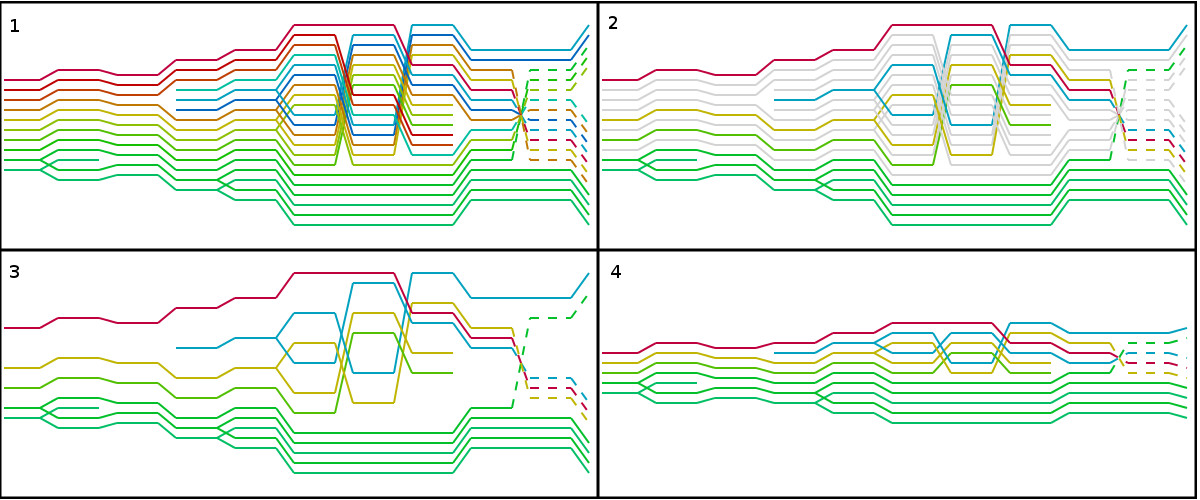
\includegraphics[width=1.1\textwidth]{images/optimalizacia}
\caption{Priebeh výberu génov}\label{obr:opt}
\end{figure}

